\documentclass{article}
\usepackage[utf8]{inputenc}

\usepackage{graphicx}
\graphicspath{{images/}}

\usepackage{float}
\usepackage{caption}
\usepackage{subcaption}
\captionsetup{compatibility=false}

\usepackage{hyperref}
\hypersetup{
    colorlinks,
    citecolor=black,
    filecolor=black,
    linkcolor=black,
    urlcolor=blue
}

\title{Polytope}
\author{URL, Mathtician, }
\date{February 2021}

\begin{document}

\maketitle

\section{Introduction}
Welcome to the \href{https://discord.gg/invite/zMRu7T4}{Polytope Discord}!

\subsection{What is a polytope?}
A \textbf{polytope} is a general name for
\textbf{polygons} (2D), \textbf{polyhedra} (3D), \textbf{polychora} (4D),
and so on for any dimension.
As with many of the terms that the Polytope Discord uses,
the word ``polytope'' can have a few definitions which are not completely equivalent.
All of the commonly-used ones, however, agree on the following:
\begin{itemize}
\item A polytope in $n$ dimensions (known hereafter as an $n$-polytope)
  is made of \textbf{facets} which are $(n-1)$-polytopes.\\
  Polychora ($4$-polytopes) are made of polyhedra ($3$-polytopes),\\
  which are made of polygons ($2$-polytopes),\\
  which are made of line segments ($1$-polytopes),\\
  which are made of points ($0$-polytopes)!
\end{itemize}

\section{Regular polytopes}
There are multiple definitions for when a polytope is \textbf{regular},
but they all require every element (vertices, edges, faces, etc.) to ``look the same.''

\section{Uniform polytopes}
General polytopes can be very complicated. Therefore, we only tend to study specific categories of polytopes. The type of polytopes we study most in this server are \textbf{uniform polytopes}.

Uniformity is defined recursively. In 2D, uniform polytopes are simply the regular polygons.
In higher dimensions, uniform polytopes are the vertex-transitive polytopes whose facets are all uniform. To see what we mean, let's look at a few examples.

\begin{figure}[H]
\centering
\begin{subfigure}{.33333\textwidth}
  \centering
  \includegraphics[width=.5\linewidth]{tut}
  \caption{Truncated tetrahedron\\(tut)}
  \label{fig:tut}
\end{subfigure}%
\begin{subfigure}{.33333\textwidth}
  \centering
  \includegraphics[width=.5\linewidth]{did}
  \caption{Dodecadodecahedron\\(did)}
  \label{fig:did}
\end{subfigure}%
\begin{subfigure}{.33333\textwidth}
  \centering
  \includegraphics[width=.5\linewidth]{snid}
  \caption{Snub icosidodecahedron\\(snid)}
  \label{fig:snid}
\end{subfigure}%
\caption{Three examples of uniform polyhedra. They all have regular polygonal faces (corresponding to the 2D uniforms) and are vertex-transitive.}
\label{fig:uniforms3D}
\end{figure}

In 3D, the uniform polytopes have already been enumerated. It turns out that, aside from the infinite families of \textbf{prisms} and \textbf{antiprisms}, there's exactly 75 uniform polyhedra. % TODO: Link to a listing

\begin{figure}[H]
\centering
\begin{subfigure}{.5\textwidth}
  \centering
  \includegraphics[width=.5\linewidth]{hep}
  \caption{Heptagonal prism (hep)}
  \label{fig:hep}
\end{subfigure}%
\begin{subfigure}{.5\textwidth}
  \centering
  \includegraphics[width=.5\linewidth]{heap}
  \caption{Heptagonal antiprism (heap)}
  \label{fig:heap}
\end{subfigure}%
\caption{An example of a prism and an antiprism. These can be built from any regular polygon, and made uniform in all cases.}
\label{fig:prisms}
\end{figure}

In 4D and higher up, the problem of enumerating the uniforms remains unsolved. As of February 2021, we know of two infinte families plus 2194 uniform polychora. In 5D and up, we haven't yet done a thorough examination, though we know of various constructions that generate uniforms in any dimension.

\subsection{Coxeter Diagrams}


\subsection{Multiprisms}

\section{CRF polytopes}
A polytope is called \textbf{convex regular-faced}, or \textbf{CRF} for short, when it is convex (without dents, holes or self-intersections) and all of its faces are regular. Let's look at a few examples.

\begin{figure}[h]
\centering
\begin{subfigure}{.33333\textwidth}
  \centering
  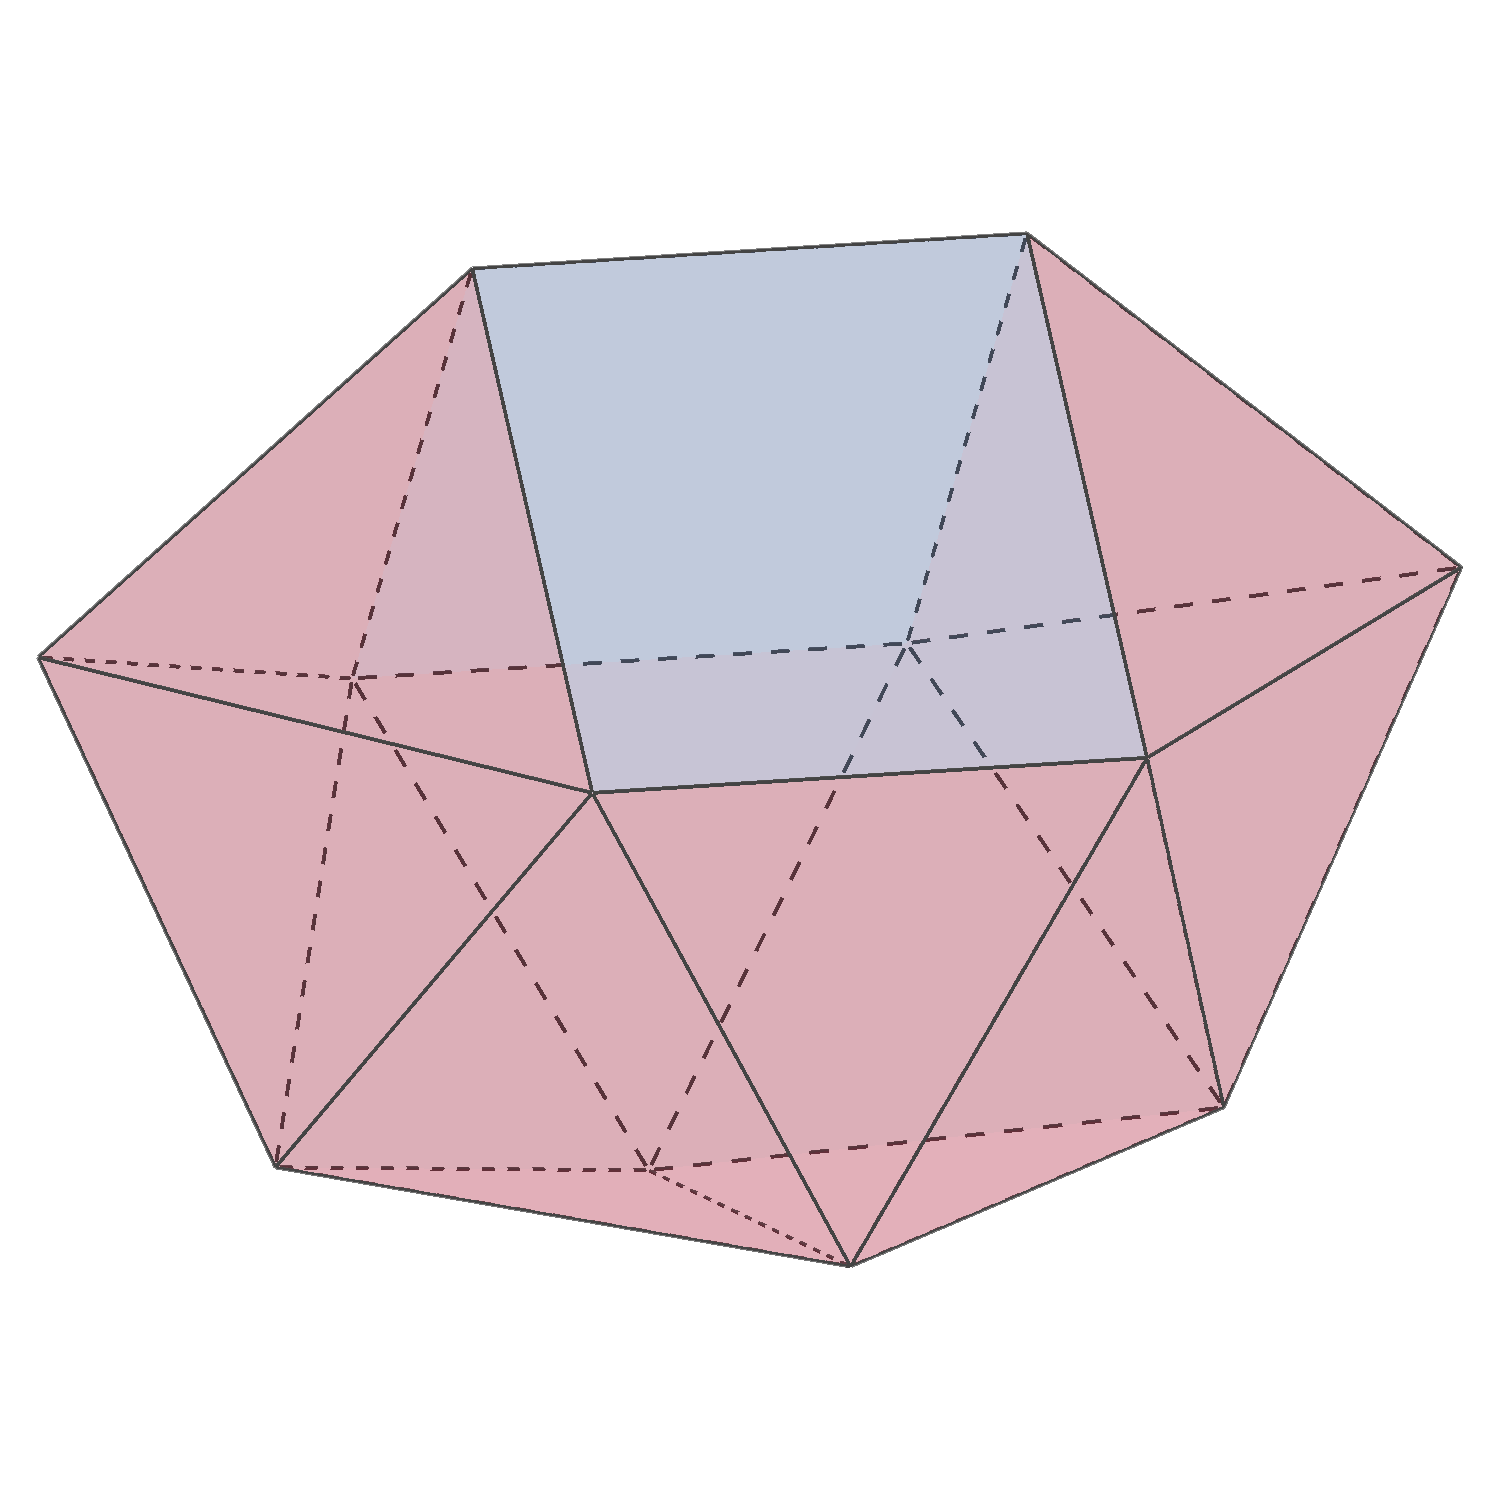
\includegraphics[width=.5\linewidth]{Sphenomegacorona}
  \caption{Sphenomegacorona}
  \label{fig:polyhedra_1}
\end{subfigure}%
\begin{subfigure}{.33333\textwidth}
  \centering
  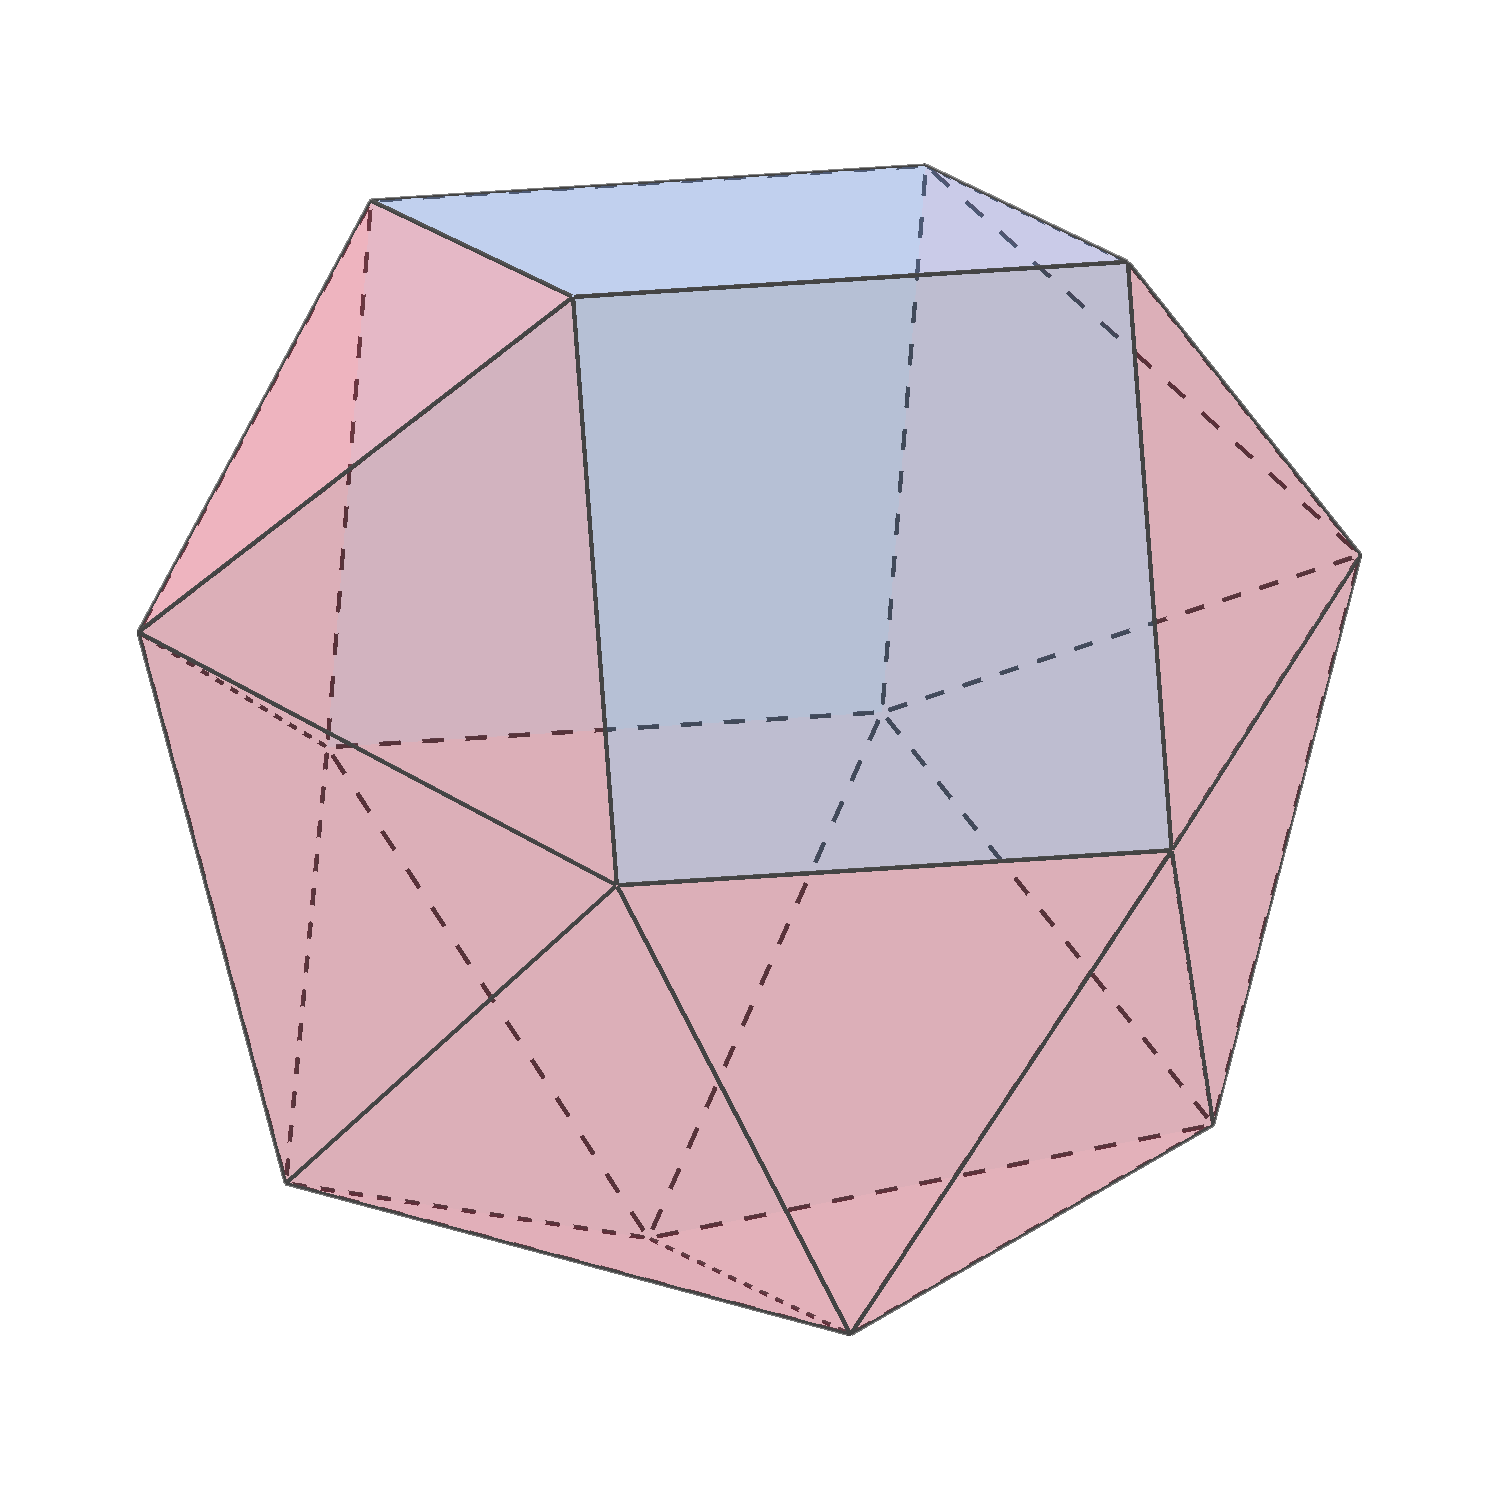
\includegraphics[width=.5\linewidth]{Hebesphenomegacorona}
  \caption{Hebesphenomegacorona}
  \label{fig:polyhedra_2}
\end{subfigure}%
\begin{subfigure}{.33333\textwidth}
  \centering
  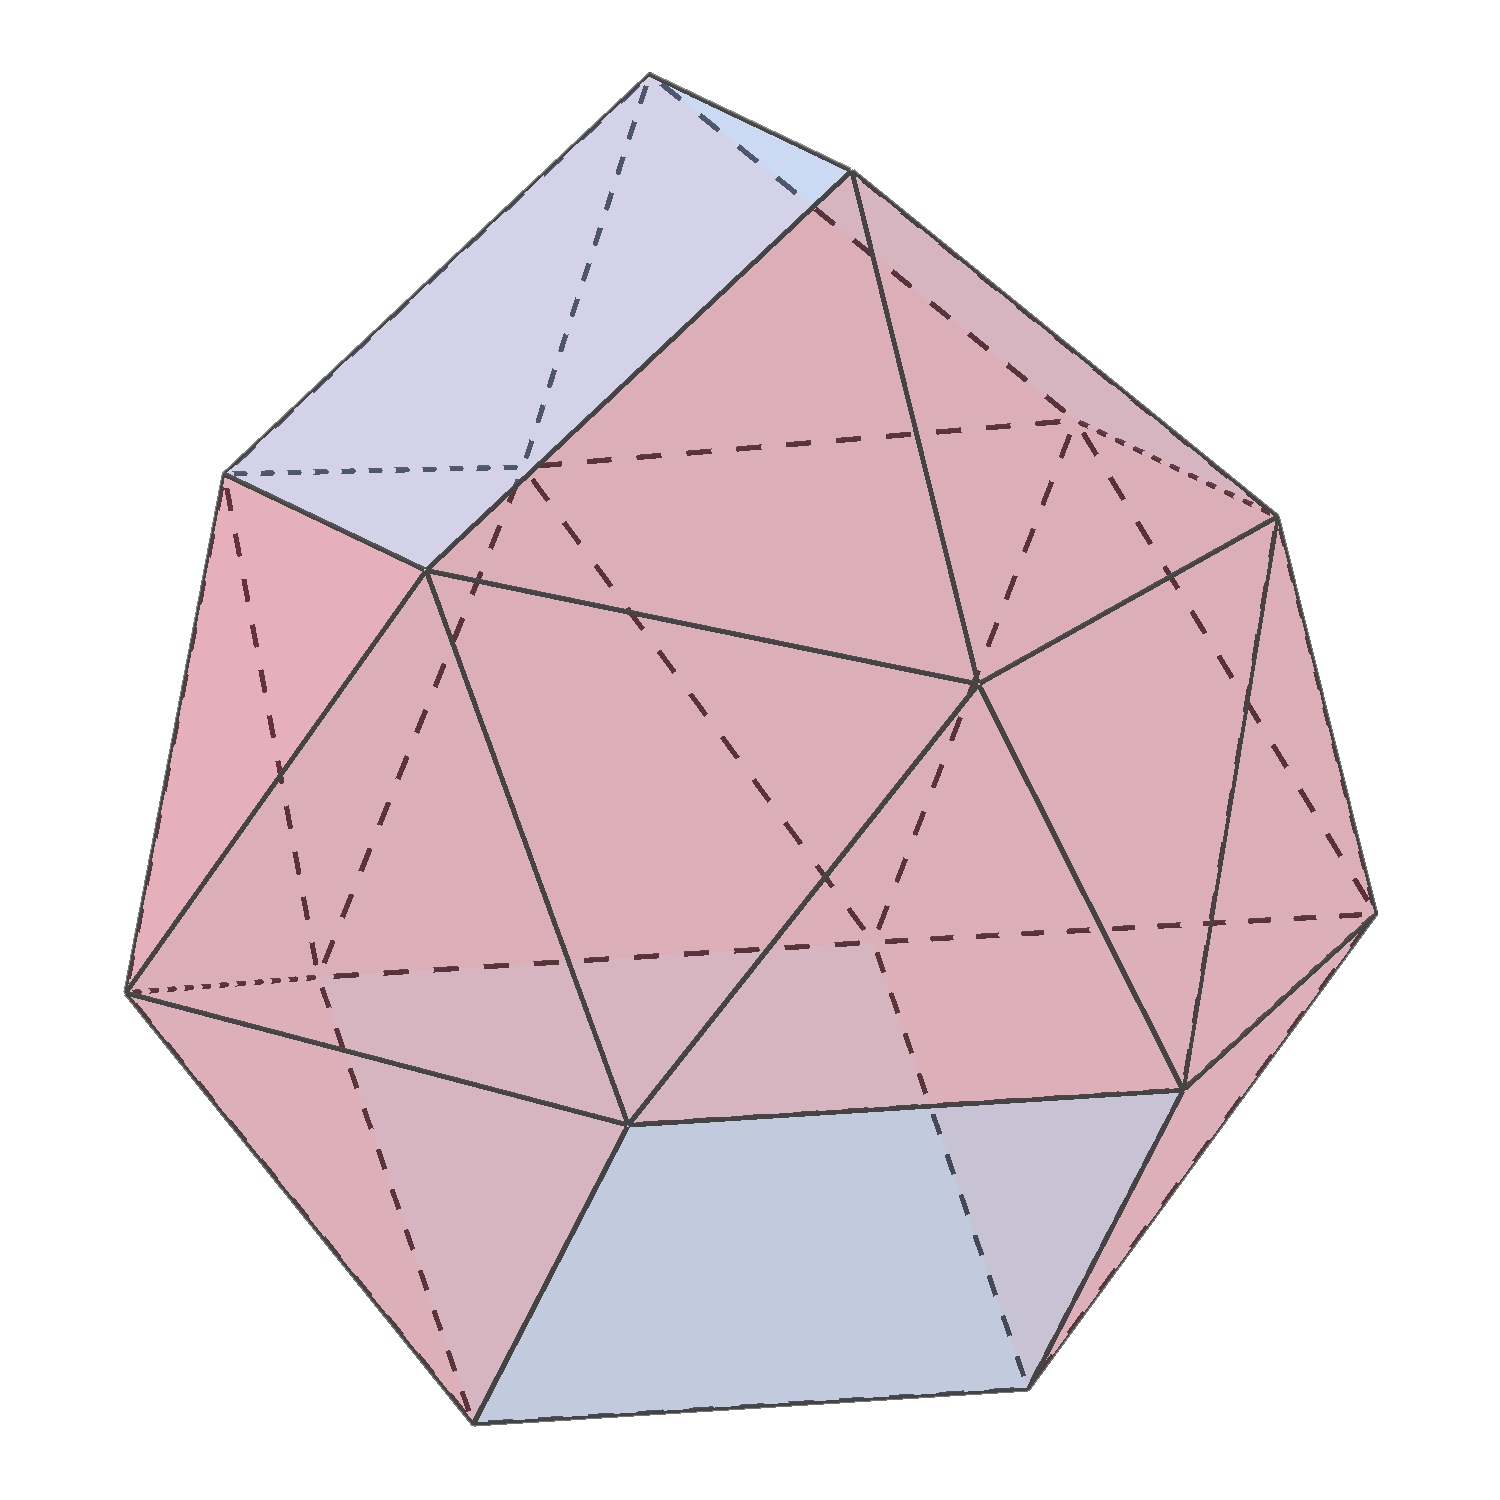
\includegraphics[width=.5\linewidth]{Disphenocingulum}
  \caption{Disphenocingulum}
  \label{fig:polyhedra_3}
\end{subfigure}%
\caption{Test images!}
\label{fig:polyhedra}
\end{figure}


\end{document}
